\section{Motivation}

\begin{figure}
  \centering
    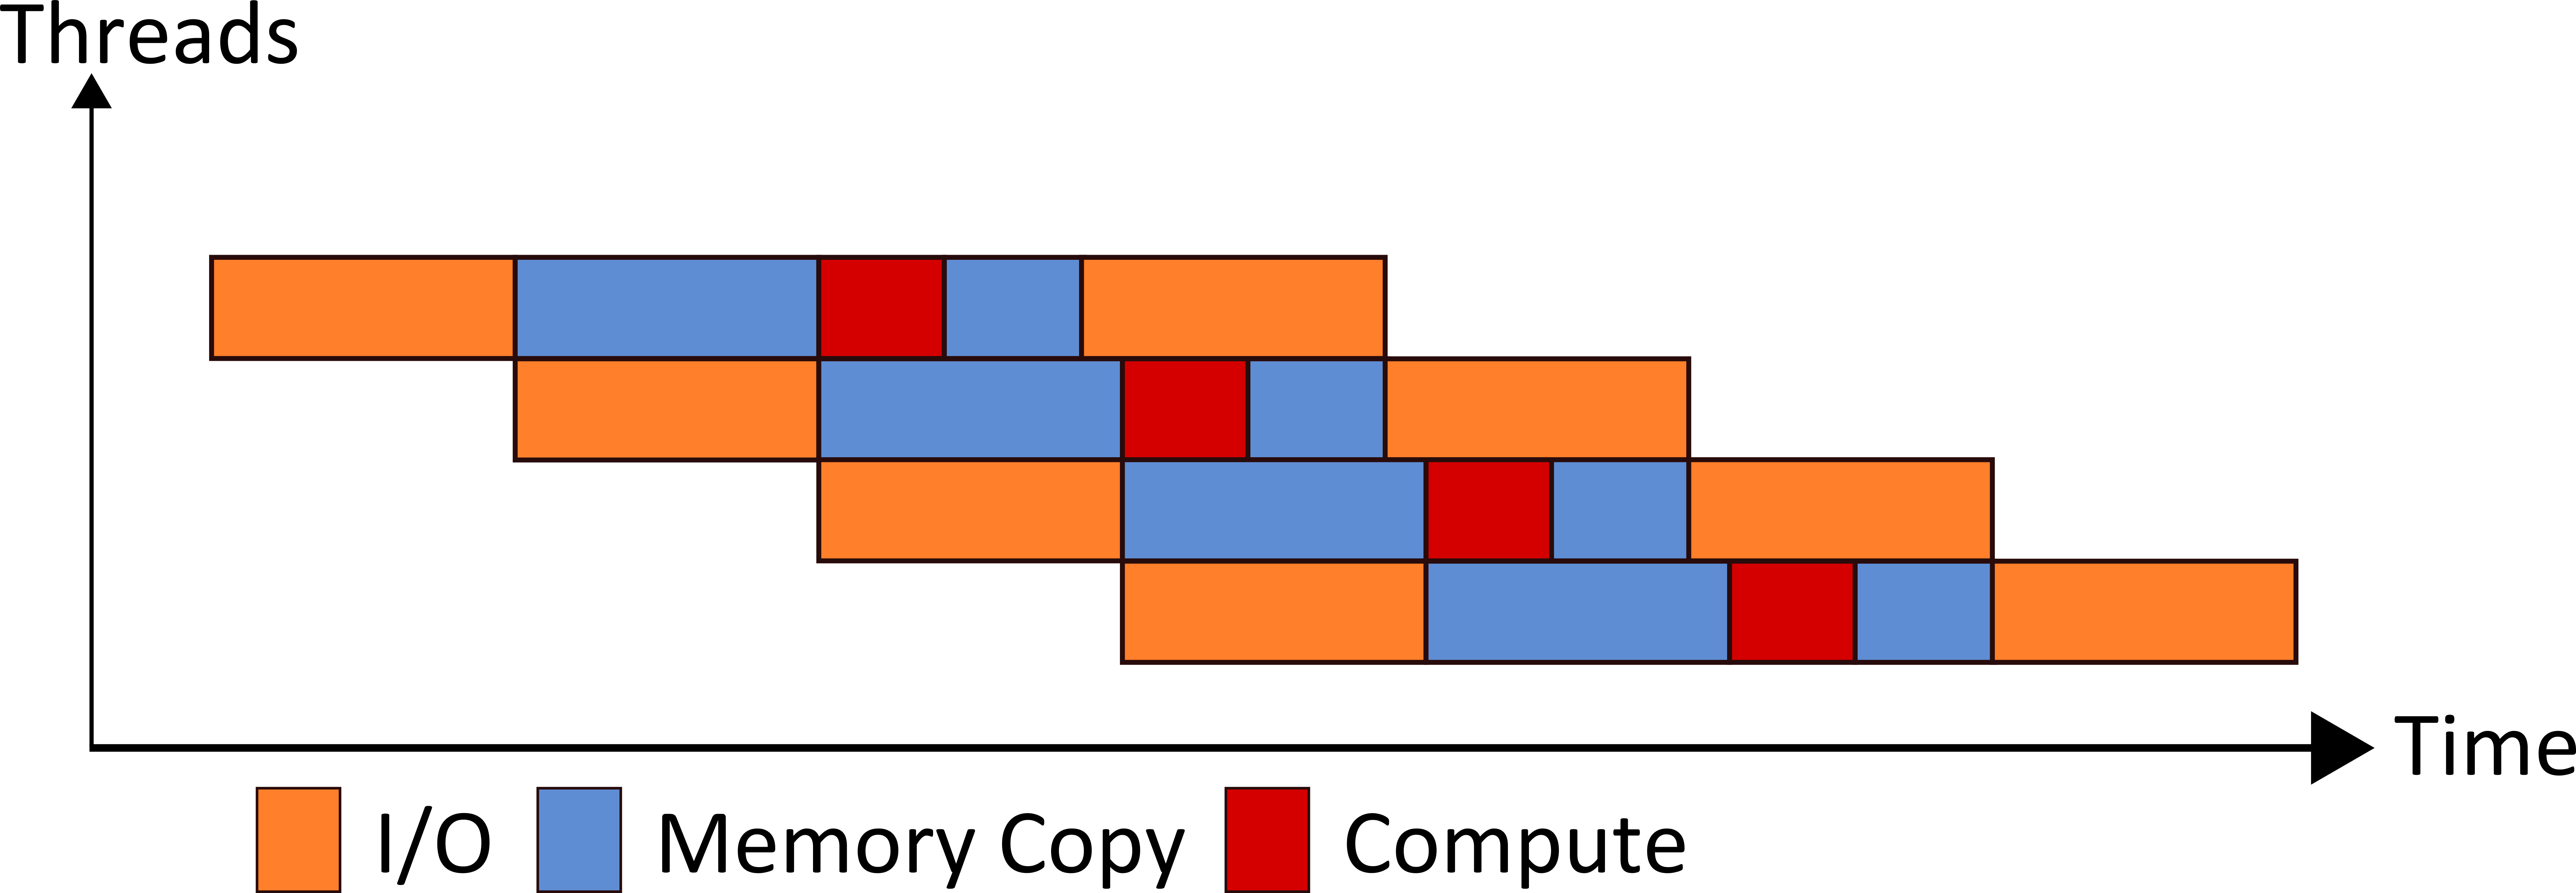
\includegraphics[width=0.5\textwidth]{fig/ord.png}
  \caption{A representation of simple overlap of host I/O, host-to-device data
           transfer, and kernel execution. In this example, there are no
           dependencies between kernels and data so management is relateively
           simple.}
  \label{fig:ord}
\end{figure}

\begin{figure}
  \centering
    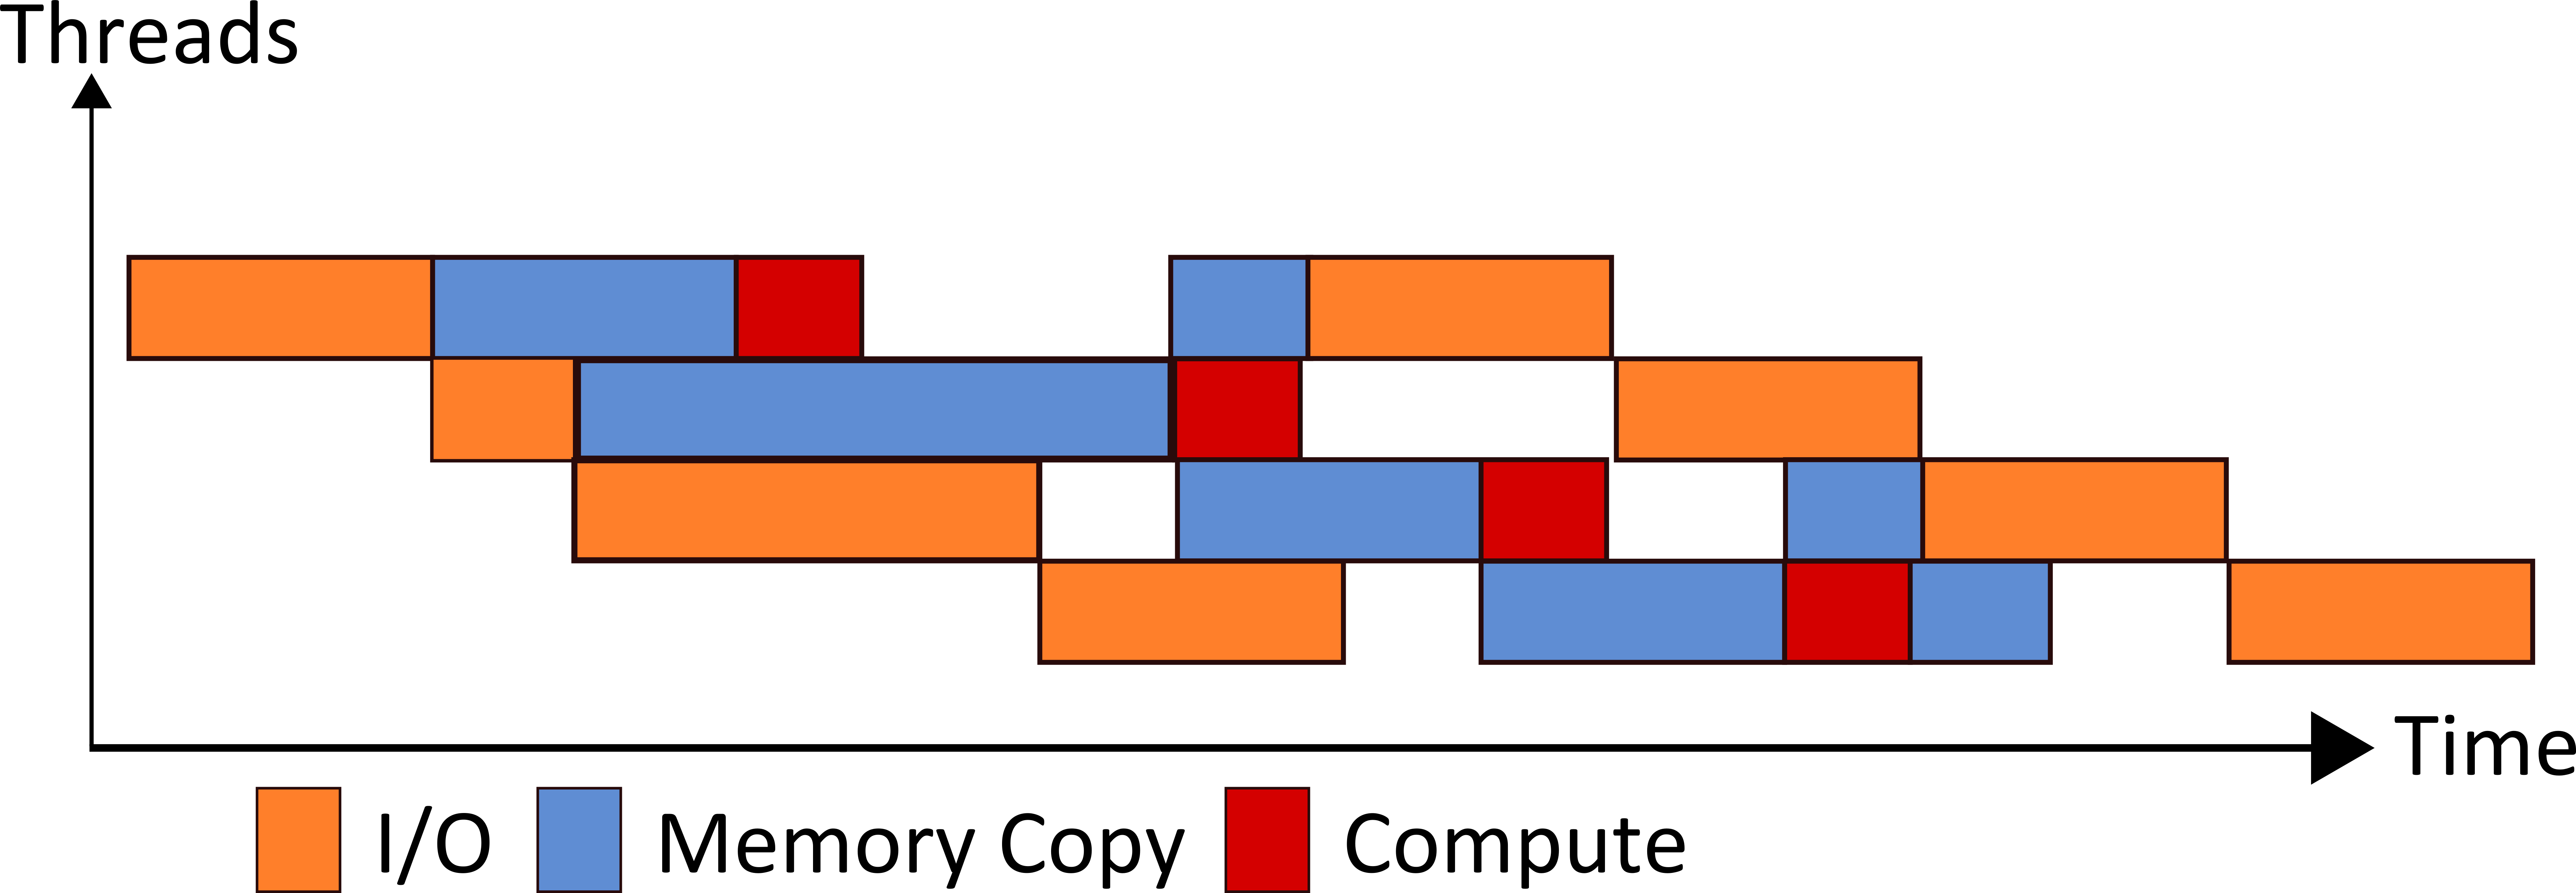
\includegraphics[width=0.5\textwidth]{fig/unord.png}
  \caption{A more complicated oververlap of host I/O, host-to-device data
           transfer, and kernel execution. Arbitrary data-dependence between
           kernels and transfers places too large a burden on the programmer
           to manage properly.}
  \label{fig:unord}
\end{figure}

When using GPUs to process big data, two major sources of latency are disk I/O
and data transfer between the host and device. OpenCL and CUDA provide methods
for managing simple patterns of overlap of data transfer and compute, shown in
Figure~\ref{fig:ord}. However, this does not assist with disk I/O.
Furthermore, in more complicated programs the existing methods are difficult to
implement efficiently. 

Figure~\ref{fig:unord} shows an example of overlapping in a more complicated
program varied I/O and transfer times. These dependencies are difficult to
efficiently manage statically because the latencies may not be known ahead of
time. Runtime management of these transfers is necessary to get efficient
results.

 

